%----------------------------------------------------------------------------------------
%   PACKAGES AND OTHER DOCUMENT CONFIGURATIONS
%----------------------------------------------------------------------------------------

\documentclass[paper=a4, fontsize=11pt]{scrartcl} % A4 paper and 11pt font size

\usepackage[T1]{fontenc} % Use 8-bit encoding that has 256 glyphs
\usepackage{fourier} % Use the Adobe Utopia font for the document - comment this line to return to the LaTeX default
\usepackage[english]{babel} % English language/hyphenation
\usepackage{amsmath,amsfonts,amsthm} % Math packages
\usepackage[utf8]{inputenc}
\usepackage{ tipa }
\usepackage{lipsum} % Used for inserting dummy 'Lorem ipsum' text into the template
\usepackage{verbatim}
\usepackage{hyperref}
\usepackage{sectsty} % Allows customizing section commands
\allsectionsfont{\centering \normalfont\scshape} % Make all sections centered, the default font and small caps
\usepackage{graphicx}
\usepackage{fancyhdr} % Custom headers and footers
\pagestyle{fancyplain} % Makes all pages in the document conform to the custom headers and footers
\fancyhead{} % No page header - if you want one, create it in the same way as the footers below
\fancyfoot[L]{} % Empty left footer
\fancyfoot[C]{} % Empty center footer
\fancyfoot[R]{\thepage} % Page numbering for right footer
\renewcommand{\headrulewidth}{0pt} % Remove header underlines
\renewcommand{\footrulewidth}{0pt} % Remove footer underlines
\setlength{\headheight}{13.6pt} % Customize the height of the header
\usepackage{xcolor}
\numberwithin{equation}{section} % Number equations within sections (i.e. 1.1, 1.2, 2.1, 2.2 instead of 1, 2, 3, 4)
\numberwithin{figure}{section} % Number figures within sections (i.e. 1.1, 1.2, 2.1, 2.2 instead of 1, 2, 3, 4)
\numberwithin{table}{section} % Number tables within sections (i.e. 1.1, 1.2, 2.1, 2.2 instead of 1, 2, 3, 4)

\setlength\parindent{0pt} % Removes all indentation from paragraphs - comment this line for an assignment with lots of text
\usepackage{fancyvrb}
\usepackage{anysize}
\marginsize{2cm}{2cm}{1cm}{1cm}
%----------------------------------------------------------------------------------------
%   TITLE SECTION
%----------------------------------------------------------------------------------------

\newcommand{\horrule}[1]{\rule{\linewidth}{#1}} % Create horizontal rule command with 1 argument of height

\title{   
\normalfont \normalsize 
\textsc{Facultad de Ciencias Exactas, Ingeniería y Agrimensura} \\ [25pt] % Your university, school and/or department name(s)
\horrule{0.5pt} \\[0.4cm] % Thin top horizontal rule
\huge Aprendiendo a pronunciar texto en Inglés \\ % The assignment title \\
\horrule{2pt} \\[0.5cm] % Thick bottom horizontal rule
}

\author{Jeremías Rodríguez} % Your name

\date{\normalsize\today} % Today's date or a custom date

\begin{document}

\maketitle % Print the title

%----------------------------------------------------------------------------------------
%   PROBLEM 1
%----------------------------------------------------------------------------------------

\section{Introducción}

\par La pronunciación del lenguaje inglés ha sido estudiada extensivamente por lingüistas, y mucho es sabido sobre las correspondencias entre letras y los sonidos del habla inglesa, llamados \emph{fonemas}.  El inglés es un lenguaje particularmente difícil de dominar por sus irregularidades en la pronunciación. Por ejemplo, la letra "a" en la palabra "gave" es una vocal larga,  pero no en "have" o "read".\\
\par En este trabajo se busca aplicar varios de los contenidos estudiados en este curso (y el anterior) al problema de convertir texto en inglés a su correspondiente transcripción en fonemas\footnote{El Alfabeto Fonético Internacional es un sistema de notación fonética creado por lingüistas. Su propósito es otorgar, de forma regularizada, precisa y única, la representación de los sonidos de cualquier lenguaje oral. Tiene aproximadamente 107 símbolos básicos, y cada idioma hace uso de un subconjunto particular.}. \\

\begin{figure}[h!]
\centering
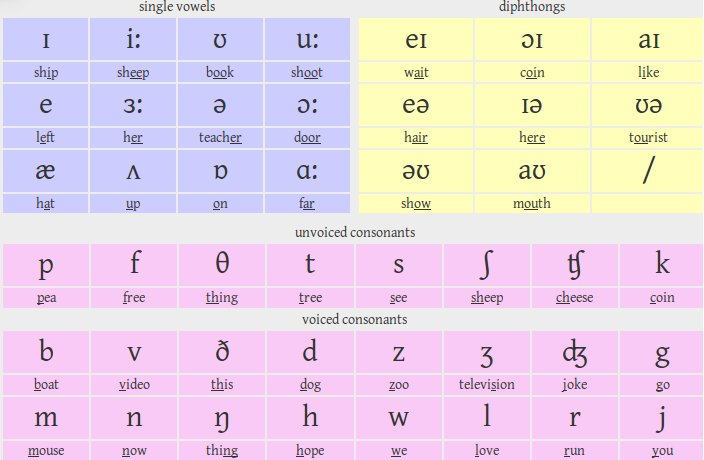
\includegraphics[width=120mm]{phonemicChart.jpg}
\caption{Algunos de los 51 fonemas del inglés oral.}
\label{fig:method}
\end{figure}

\par El dataset utilizado, llamado netTalk\footnote{\url{https://archive.ics.uci.edu/ml/datasets/Connectionist+Bench+(Nettalk+Corpus)}}, fue usado por primera vez en el paper  "Parallel Networks that Learn to Pronounce English Text"\cite{parallel}. Los autores entrenaron redes neuronales capaces de convertir strings de texto en inglés (e.g. \textit{arithmetical}) en strings de fonemas (\textit{@rIT-mEtIk-L}).\\


	

    

\par En este trabajo recrearé y analizaré varios experimentos llevados a cabo en el citado paper (con ANNs). Posteriormente aplicaré otros clasificadores (Random Forest, Gaussian Process, SVM y KNN) y compararé resultados.

\section{Dataset NetTalk}

\subsection{Presentación del dataset}
El dataset netTalk contiene una fila por cada una de las 20000 palabras del \textit{Miriam Webster’s Pocket Dictionary}. Por cada fila, el dataset contiene sólo dos columnas: \\

\begin{center}

\begin{BVerbatim}
[written_representation] [phonemic_representation]
argue                    argY-   
argumentation            argYmxnteS-xn   
argumentative            argYmEntxtIv-   
aright                   xrA--t   
arise                    xrAz-   
aristocracy              @rxstakrxsi   
aristocrat               xrIstxkr@t   
aristocratic             xrIstxkr@tIk   
arithmetic               xrIT-mxtIk   
arithmetical             @rIT-mEtIk-L   
arithmetician            xrIT-mxtIS-xn   
\end{BVerbatim}

\end{center}

Ambas columnas son de tipo string, la primera columna sólo contiene caracteres del alfabeto inglés (abc..z), mientras que la segunda columna contiene caracteres que representan fonemas. Los autores del paper original eligieron un conjunto de 51 fonemas. (ver rawDataset/netTalk.names para mas detalle).\\

En el extracto del dataset que he mostrado podemos ver que se ha forzado una correspondencia 1-1 entre letras de la primera columna y fonemas de la segunda: cada fonema corresponde al sonido producido por una de las letras . Por ejemplo, la palabra "arithmetical": 

\begin{center}

\begin{BVerbatim}
a>@ ; r>r ; i>I ; t>T ; h>- ; m>m ; e>E ; t>t; i>I ; c>k ; a>- ; l>l               
\end{BVerbatim}

\end{center}

Los autores del paper original incluyen un fonema "vacío", representado con el símbolo '-', para indicar la ausencia de sonido. Utilizando este simbolo, se rellena las transcripciones foneticas para que tengan la misma cantidad de caracteres que la palabra original (lo cual es computacionalmente conveniente).



\subsection{Preprocesamiento}

Todos los métodos que hemos estudiado en Machine Learning y Data Mining requieren que los datos input estén expresados como una matriz numérica. El dataset netTalk que se acaba de introducir es una representación a muy alto nivel de la información que queremos utilizar, y por ello se requiere un paso de preprocesamiento importante para obtener datos numéricos con los que trabajar. \\
\newpage
Comencemos por definir claramente el problema a tratar. Deseamos hallar una función f que convierta strings con palabras en inglés, a strings con su correspondiente transcripción fonética:

\begin{align*}
  f \colon Words &\to Phonetics \\
  f("hypotenuse") &= "hApat-NYs-".
\end{align*}

Utilizando el hecho de que cada letra del input se corresponde a un fonema en el output, podemos reducir el problema a hallar el fonema correspondiente de cada letra. Es decir, deseamos obtener una función $g$ que se focalice en predecir el fonema de una sola de las letras a la vez, obviamente teniendo en cuenta el contexto (letras anteriores y siguientes) en la palabra original. Asumimos que para predecir el sonido de una letra, sólo necesitamos saber las 3 letras anteriores, la letra misma y las 3 siguientes (si las hay):


\begin{align*}
  g \colon L \times L \times L \times L \times L \times L \times L  & \to Phonems \\
  g(-,-,-,\textcolor{red}{h},y,p,o) &= h \\  
  g(-,-,h,\textcolor{red}{y},p,o,t) &= A \\
  g(-,h,y,\textcolor{red}{p},o,t,e) &= p \\
  g(h,y,p,\textcolor{red}{o},t,e,n) &= a \\
  g(y,p,o,\textcolor{red}{t},e,n,u) &= t \\
  g(p,o,t,\textcolor{red}{e},n,u,s)& = - \\
  g(o,t,e,\textcolor{red}{n},u,s,e)& = N \\
  g(t,e,n,\textcolor{red}{u},s,e,-)& = Y \\
  g(e,n,u,\textcolor{red}{s},e,-,-) &= s
\end{align*}

Por supuesto, esta ventana de 7 letras puede no ser suficiente para algunas palabras donde se necesita considerar una porción más amplia para generar una correcta pronunciación; pero en general funciona bien. Finalmente, si obtenemos esta función g, podemos derivar f aplicando sucesivamente g a cada letra del input de f. 

\begin{align*}
  f("hypotenuse") = g("---\textcolor{red}{h}ypo")  g("--h\textcolor{red}{y}pot") g("-hy\textcolor{red}{p}ote") g("hyp\textcolor{red}{o}ten")  \ldots
\end{align*}


Qué ventajas tiene g respecto a f? Al tener un input fijo de 7 caracteres y un output fijo de 1 fonema; podemos aplicar los algoritmos de machine learning que hemos estudiado (los cuales requieren inputs de longitud no variable). Además, aprender la función g es sustancialmente más fácil porque sólo se predice un caracter a la vez. \\

Por lo tanto, se convirtió el dataset netTalk a un nuevo dataset intermedio de 8 columas, donde dividimos cada palabra en varias filas como se ilustró arriba con "hypotenuse". En nuestro caso, de tener 10000 palabras pasamos a tener 146934 filas. Los scripts utilizados en esta fase pueden verse en /src/encodedDs. \\

El paso restante es codificar todos los caracteres(letras y fonemas) de las 146934 filas como números. Para codificar las \textbf{letras del input} usaremos una representación muy simple: Dado que tenemos 26 letras en el alfabeto inglés, cada letra por 26 columnas binarias 1-0. Si la primera letra era una 'j', entonces la columna 10 tendrá un 1 y las otras 25 columnas un cero. Los \textbf{fonemas output}, por otra parte, se codificarán en 18 columnas binarias (ver anexo I).\footnote{Los 50 fonemas se codifican en 18 columnas que representan "articulatory features" que los definen, como por ejemplo si tienen un tono alto, medio o bajo; si el ruido procede de la garganta, del paladar, etc; o si el ruido es con o sin voz.} \\

Por lo tanto, el dataset final de 146934 filas tendrá 26 * 7 columnas binarias representando las 7 letras input; y otras 18 columnas binarias representando el fonema output. A este dataset resultante le aplicaré distintas técnicas de aprendizaje que estudiamos en el curso.

\section{Redes Neuronales}
El primer paso fue repetir los exprimentos que se realizaron usando redes neuronales en \cite{parallel}. Para ello, utilizaré una red neuronal con 26 * 7 neuronas en la capa de entrada, y 18 en la capa de salida. 

\begin{figure}[h!]
\centering
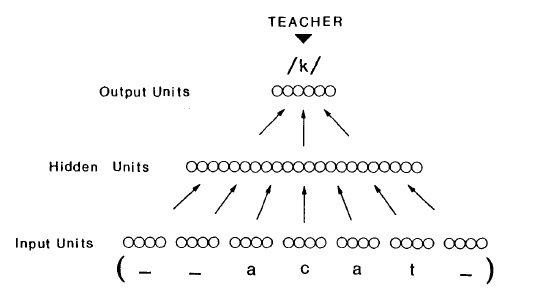
\includegraphics[width=100mm]{figure1.jpg}
\end{figure}

\subsection{Optimización de parámetros}

Para optimizar parámetros se usaron 1000 de las 20000 palabras del dataset original; divididas en 750 training y 250 validación. Realicé la búsqueda en grid search para learning rate ($\eta$) y momentum ($\mu$) entre  $10^{-1} y 10^{-5}$, y 20 neuronas intermedias. Utilicé el algoritmo backpropagation, en particular una versión modificada del codigo en C que utilizamos en el curso de machine learning. Los parámetros óptimos fueron $\mu$=0.0001 y $\eta$=0.01 y el código de toda esta sección puede verse en /src/ANNs

\begin{comment}
\begin{tabular}{ |c|c|c|c|c|c|  }
\hline
 & $\eta$ =.1 & $\eta$ =.01 & $\eta$ =.001 & $\eta$ =.0001 & $\eta$ =.00001 \\
\hline 
$\mu$ =.1     & 25.4  & 24.85 & 25.06 & 33.52 & 39.01 \\
$\mu$ =.01    & 24.92 & 24.38 & 25.18 & 33.61 & 39.94 \\
$\mu$ =.001   & 25.24 & 24.00 & 25.24 & 33.61 & 39.98 \\
$\mu$ =.0001  & 25.26 & 23.99 & 25.26 & 33.60 & 39.98 \\
$\mu$ =.00001 & 25.26 & 23.99 & 24.84 & 33.60 & 39.98 \\
\hline
\end{tabular}
\end{comment}

\subsection{Resumen de resultados usando ANNs}

\begin{figure}[h!]
\centering
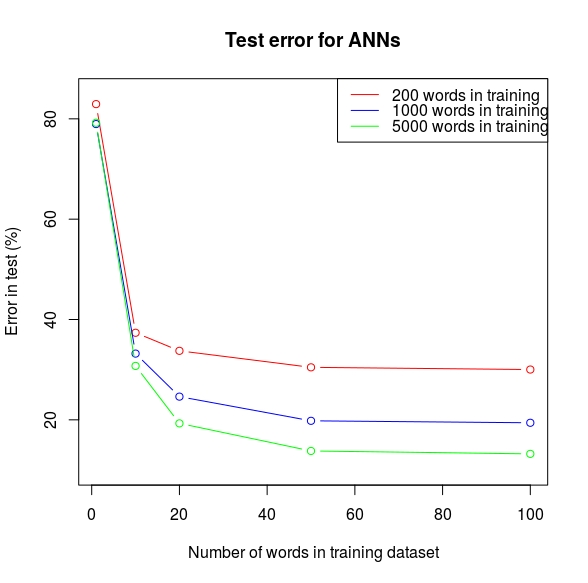
\includegraphics[width=112mm]{annresults.jpg}
\end{figure}

Una vez seleccionados los parámetros óptimos, el siguiente paso fue entrenar redes con distintas cantidades de neuronas intermedias y con distintas cantidades de puntos en training; y los resultados pueden verse en la figura anterior. \\

Algunas apreciaciones:

\begin{itemize}
\item El error usando una sola neurona intermedia es muy alto. Esto puede indicar que el problema que se está atacando es altamente no lineal.
\item Como vemos, usando una red con 20 o más neuronas podemos llegar a un accuracy muy bueno, donde más del 80\% de los fonemas son generados correctamente. El mejor error en test se obtiene con 5000 palabras en training y 100 neuronas, donde el 86.78\% de los fonemas son generados correctamente.
\item La ganancia de seguir agregando más palabras al dataset de entrenamiento se reduce cada vez más a medida que llegamos a unas 5000 palabras. 
\item A partir de 50 neuronas en adelante, continuar agregando más neuronas tampoco mejora el resultado. Apartentemente no queda más información que pueda ser aprendida por una ANN llegado a ese punto, independientemente de la complejidad de la red. Entrenar una red a'un más poderosa (150 neuronas ocultas) nos permite ver como el modelo rápidamente empieza a overfittear, llevando el error de training al 3\% pero perdiendo generalidad.
\end{itemize}

\begin{figure}[h!]
\centering
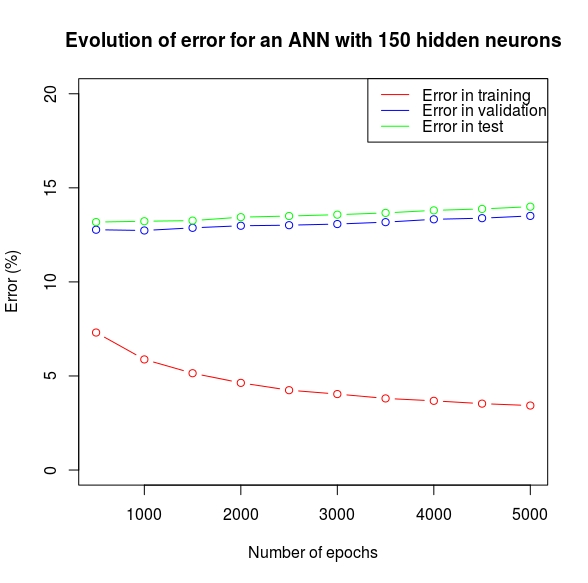
\includegraphics[width=112mm]{annresults2.jpg}
\end{figure}

Este "estancamiento" en la reducción del error (descripto en los ultimos dos items) probablemente se deba a que:

\begin{itemize}
\item Hay irregularidades y excepciones del lenguaje que no puedan ser deducidas a partir de otros ejemplos de entrenamiento. Es necesario memorizar cada uno de esos casos por separado.
\item Estamos usando una ventana de 7 caracteres para pronunciar, y probablemente hay palabras cuyos patrones de pronunciación podrían ser aprendidos considerando una ventana mayor.
\end{itemize}


Me parece asombroso llegar a predecir con tanta exactitud los fonemas, dado que este problema es muy complejo, altamente dimensional y posee una gran cantidad de reglas y excepciones. \\

Lo que más me sorprende de estos resultados es que con sólo 200 palabras de ejemplo del idioma somos capaces de predecir la pronunciación del resto del idioma con casi 80\% de precisión (habilidad que a un ser humano puede llevarle realmente mucho tiempo y muchos más ejemplos adquirir). \\


\subsection{Ejemplos de output}

\begin{center}
\begin{BVerbatim}
Written Representation  predicted Phonetics   real Phonetics  
machine                 m@C-en-               mxS-in-  
learning                lI-rnIG-              l--RnIG- 
unexpected              xnEXpEktxd            xnIXpEktxd  
beautiful               bcc-tIfcl             bY--tIf^l 
telescope               tIlEskxp-             tElxskop- 
virus                   varxs                 vArxs

\end{BVerbatim}
\end{center}


Como se puede apreciar, la red se confunde en varios fonemas, pero los errores son muy similares a los que cometemos las personas, pues la confusión se da generalmente entre vocales con sonidos similares. \\

\section{ Otros métodos de machine learning }


Me interesa analizar ahora la performance de otros algoritmos que hemos estudiado en el curso, y compararla con los resultados vistos en la sección anterior. Los métodos que decidí aplicar a este problema de clasificación son Nearest Neighbor, Random Forest, SVM y Gaussian Processes. Los resultados pueden observarse en la Figura 4.1, y a continuación comentarios de implementación y conclusiones:


\begin{itemize}
\item \textbf{Nearest Neighbor}: Decidí usar este método simple para obtener un "baseline" del error, calculando Nearest Neighbor usando sólo la letra central. Por ejemplo, si deseamos predecir el fonema generado por el input (y,p,o,\textcolor{red}{t},e,n,u), se descartan las columnas de contexto y simplemente se busca en el dataset de training otro input donde la letra a predecir sea tambien \textcolor{red}{t}. Encontrado este nearest neighbor en train (por ejemplo, (w,a,n,\textcolor{red}{t},-,-,-) , se retorna el fonema asociado \textcolor{red}{t}.

Como era de esperar, aproximadamente la mitad de los fonemas son predichos correctamente. Estos fonemas corresponden principalmente a consonantes cuya pronunciacion es generalmente constante. Este método tiene la desventaja de qué el tiempo de predicción es muy alto pues hay que recorrer todo el dataset.

\item \textbf{Nearest Neighbor sílaba}: Similar al anterior. En este caso, si deseamos predecir el fonema generado por el input (y,p,o,\textcolor{red}{t},e,n,u), buscamos el nearest neighbor en train usando las tres columnas centrales (o,\textcolor{red}{t},e). De esta forma, se busca una sílaba en train que sea parecida a la sílaba que queremos predecir. Me sorprendió descubrir que el error obtenido por este método rivaliza a los otros metodos, siendo los demas mucho más sofisticados. El salto de accuracy entre NN y NN-silabico demuestra la importancia de tener en cuenta el contexto de una letra a la hora de generar su fonema.

Una desventaja de este approach es el tiempo que se tarda para realizar una prediccion, lo cual lo hace inadecuado para aplicaciones que generen sonidos en tiempo real. 

Además vemos que al quintuplicar el tamanyo del dataset de train (1000 a 5000), no se ve un gran incremento en la reducción del error. Mi hipótesis es que esto sucede porque este método es incapaz de hacer algún aprendizaje real o inteligente, sólo busca sílabas similares, y esta forma de operar no permite descubrir conexiones mas complejas entre inputs y outputs. Pronunciaciones de vocales que sigan patrones mas sofisticados, o fonemas que requieran de un contexto mayor, no serán predichos correctamente.

\item \textbf{Random Forest}: Dado que hay 18 columnas binarias de output, entrené 18 clasificadores RF, cada uno especializado en predecir la columna de output i-ésima. Utilicé 500 árboles por ensemble.

En mi opinion este es el mejor método de los que he experimentado. Si bien ANN con 50 neuronas es un poco mas preciso, el tiempo consumido para entrenar los 20 clasificadores random forest es menor que el de entrenar la red neuronal. Ademas, RF fue extremadamente sencillo de usar, pues no requirió optimizar hiperparámetros.

Cada nodo en cada árbol de decisión supongo que significará una regla especial para una determinada letra, dado que cada input tiene valor 0 o 1 (no hay mas variacion que esa). Por lo tanto, cuando los árboles de decisión intenten hacer "cortes", representarán decisiones a tomar de acuerdo a si un particular input esta encendido o apagado (0-1), es decir, de acuerdo a si el input es una letra en particular o no.

\item \textbf{SVM}: Al igual que con RF, entrené 18 clasificadores, cada uno especializado en predecir la columna de output i-ésima. Use un kernel Gaussiano, lo cual involucra la dificultad extra de optimizar hiperparámetros. Para cada una de las 18 columnas, optimice $C$ y $\sigma$ en grid search.

El problema es altamente dimensional y no lineal, por lo que la posibilidad de usar el kernel trick es muy valiosa. Optimizar los hiperparámetros a medida que el dataset crece se vuelve muy costoso computacionalmente, pero se reflejo en mejoras de aproximadamente 5\%.

\item \textbf{Gaussian Processes}: Si bien no estudiamos este método en el curso, me pareció interesante incluirlo\cite{gauss_processes}. Al igual que para SVM y RF, este método sirve para clasificación y regresión, y tuve que entrenar un clasificador por columna. 

Otra similitud de este método con SVM es la posibilidad de aplicar el kernel trick. El kernel usado es Gaussiano, aunque la optimización de hiperparámetros es realizada automáticamente por kernlab (ya que puede estimarse maximizando el likelihood de los datos de train).

Una ventaja de este método es que cada predicción tiene una varianza asociada, que nos permite medir cuan confiable es la predicción.

Sin embargo, este método probó no ser nada adecuado para este problema. En primer lugar, dado que se necesita mantener una matriz de $n^2$ puntos en memoria donde n es el valor de training, el consumo de memoria resultó tan prohibitivo que no pude realizar los cálculos para n~40000 (5000 palabras). Una de las principales ventajas de GPs es que son muy buenos interpolando datos continuos en áreas donde no hay mucha información, pero esta ventaja no es aprovechada en este problema.

\item \textbf{ANNs} Las redes neuronales dieron los mejores resultados. Esta tarea de aprendizaje complejo, en donde el output es claramente una funcion no linear de los inputs, es adecuada para la potencia de redes neuronales. Las redes se benefician de que tenemos una gran cantidad de datos de entrenamiento. A diferencia de los otros clasificadores, hubo que entrenar una sola red con 18 outputs; mientras que todos los demás clasificadores (excepto KNN) requirieron entrenar 18 clasificadores diferentes.

\end{itemize}



\begin{center}
\begin{figure}[h!]
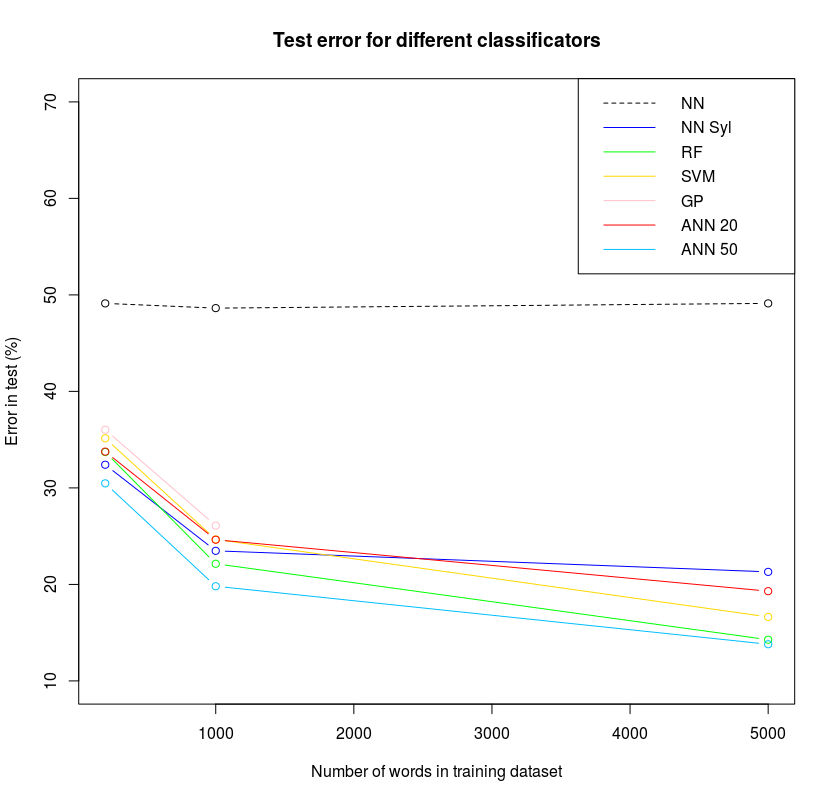
\includegraphics[width=170mm]{figure.png}
\caption{Error en test para distintos clasificadores}
\label{fig:results}

\end{figure}
\end{center}

\newpage

\section{ Importancia de variables input}

No pude aplicar técnicas de clustering/reducción de dimensionalidad debido a que no tienen sentido para la codificación en columnas binarias del dataset. Los métodos que estudiamos no tienen forma de saber que en mi codificación, la letra central es la mas importante y las otras 6 letras son contexto. Tampoco tienen forma de saber que los inputs estan agrupados en 7 grupos de 26. \\

Para compensar la falta esos análisis en este trabajo, y dado que Random Forest es uno de los algoritmos que dio mejores resultados, decidí aprovechar su capacidad de asignar una importancia a las variables inputs. Esto me permitirá aprender un poco más sobre cuáles inputs son mas importantes para generar los sonidos del idioma. \\

Para hacer este pequeño experimento, usé un dataset de training de 200 palabras y entrene 18 clasificadores RF (uno por cada feature del output). Recordemos que los 18 outputs son columnas binarias que indican la presencia o ausencia de una particular característica en sonido del fonema. Por ejemplo: nasal, labial; alto, bajo ; líquido, etc. \\

Para cada uno de estos 18 clasificadores RF que entrené, consulté cuales eran las 26 columnas input mas importantes. Recordemos que el dataset tiene 26*7 columnas input, cada grupo de 26 codifica una de las letras input. El resultado que espero es que las 26 columnas que codifican la letra central sean las más importantes, seguidas por las columnas que codifican la letra inmediata anterior y siguiente. \\

Cada uno de los 18 clasificadores dio su ranking de los 26 inputs mas importantes, y el siguiente histograma intenta agrupar los resultados:

\begin{figure}[h!]
\centering
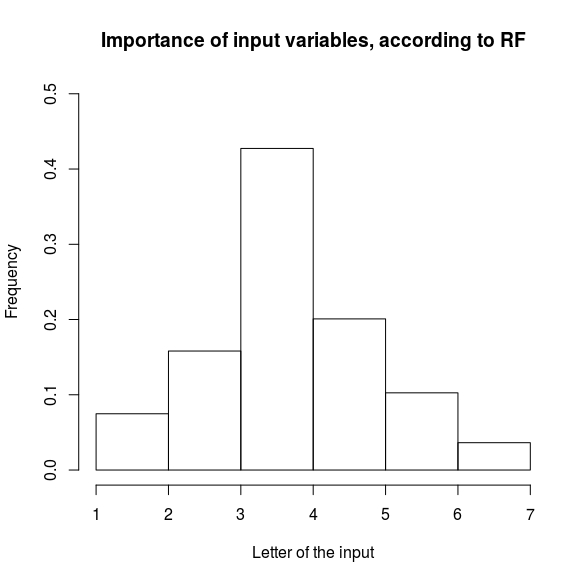
\includegraphics[width=100mm]{variable_importance.jpg}
\caption{En el eje x se agrupo los 26*7 inputs en 7 barras de histograma. La altura representa la cantidad de ocurrencias de una de las variables del grupo i-ésimo como parte de las 26 variablas más importantes, de acuerdo a los 18 predictores RF.}
\label{fig:results}

\end{figure}

En el histograma podemos observar que la letra central es la más importante a la hora de predecir las caracterásticas del fonema output. Sin embargo, hubiese esperado que la importancia de la letra central fuese mucho más determinante. De acuerdo a RF, la letra anterior y siguiente a la letra central son de vital importancia. \\

Me resulta muy curioso que la quinta letra (la siguiente a la letra central) sea mas importante para determinar la pronunciación que la tercera. Para verificar que no es un error aleatorio, repeti el experimento con distintos datasets de train, y aún así observé la misma tendencia. \\

Además, pude observar otras regularidades mirando de a un output a la vez. Tomemos por ejemplo la columna de output 8, que singifica "fonema nasal" (el fonema predicho tendra un sonido nasal). Sabemos, por la tabla del anexo 1, que los fonemas asociados a sonidos nasales son "m", "n", "G","J","M","N". Letras que usualmente generan estos sonidos son "m" y "n". \\

De acuerdo a random forest, las cinco variables input más importantes para detectar si un fonema es nasal son:

\begin{center}
[1]  92  91  83  85  87
\end{center}

Que corresponden a letras centrales n, m, e, g, i. Esto nos demuestra que random forest es suficientemente inteligente para descubrir estas conexiones entre letras del input y particulares características de su pronunciacion. Este tipo de conexiones es imposible de descubrir por algoritmos básicos como KNN.

\section{ Reflexión final }

Los distintos métodos de machine learning que estudiamos en estos dos cursos dieron resultados muy buenos en el dataset NetTalk, con errores en test bastante similares. Todos resultaron muy costosos computacionalmente, tardando horas y horas en realizar las predicciones. \\

Hacer este trabajo me resultó muy interesante, no sólo porque me apasiona el campo de machine learning, si no que también por que me permitió aprender sobre lenguajes que es otro campo muy interesante. \\

En el caso particular del idioma inglés, la aplicación práctica de estos metodos puede no ser muy amplia dado que es un lenguaje extensamente estudidado y probablemente un sistema con reglas pueda tener mayor performance. \\

Sin embargo, imagino que este mismo procedimiento (aprender la pronunciación desde ejemplos) funcionaría para aprender cualquier idioma, provisto un dataset de palabras y sus transcripciones fonéticas. Esto es muy interesante, porque partiendo de una pequeña muestra de palabras, podriamos aproximar bastante bien la pronunciacion del lenguaje. \\

Estos métodos podrían ser usados en el estudio de lenguajes vivos pero poco estudiados, lenguajes antiguos o incluso semi-extinguidos. Si sólo se conoce la pronunciacion de un subconjunto de palabras del lenguaje, podría ser posible aplicar estos metodos para predecir como seria la pronunciacion del lenguaje completo. \\






\newpage

\section { Anexo I: Articulatory Features}


\begin{center}
\begin{figure}[h!]
\centering
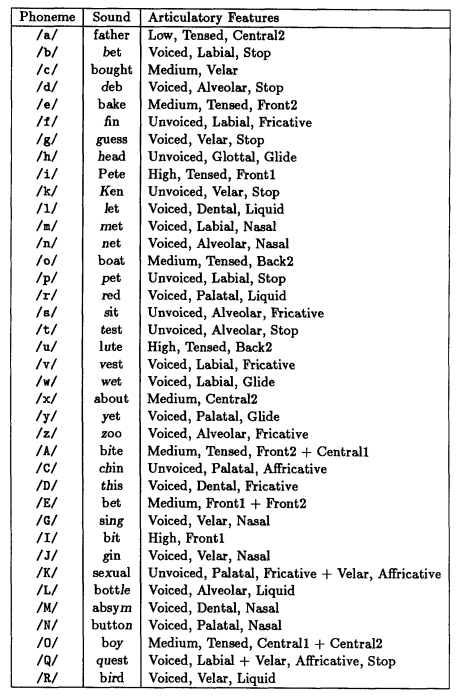
\includegraphics[width=100mm]{art_features.jpg}
\end{figure}
\end{center}

\begin{center}
\begin{figure}[h!]
\centering

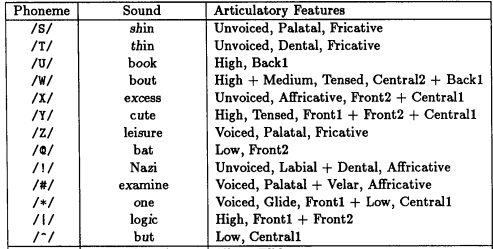
\includegraphics[width=100mm]{art_features2.jpg}
\end{figure}
\end{center}



\begin{thebibliography}{9}
\bibitem{parallel} 
Terrence J. Sejnowski and Charles R. Rosenberg
\textit{Parallel Networks that Learn to Pronounce English Text}. 
Complex Systems 1 (1987)

\bibitem{gauss_processes} 
Book by Carl Edward Rasmussen and Christopher K. I. Williams\textit{ Gaussian Processes for Machine Learning}. 



\end{thebibliography}

\end{document}
